%\newpage

\section{Inertial Range}\label{appInertial}


For our analysis it is essential to verify that there is a reasonable range of scales $\ell$ below the driving range within which the simulations are not dominated by numerical effects, so that they resolve the inertial range of any turbulent cascade.  
We note that the fitting region for our VSFs starts at lags greater than eight zones, ensuring that the numerical dissipation range lies at smaller scales.
To understand the non-power law behaviour that we nonetheless find, in the following subsections we offer more examples that show VSFs of all three clouds at different times and considering our different analysis approaches. 
We focus on the standard analysis in Sect.~\ref{Bsub:standard}, on the
analysis neglecting the density threshold in Sect.~\ref{Bsub:full},
and on the impact of varying the resolution in collapsing regions in Sect.~\ref{Bsub:Jeans}.

 	
\begin{figure*}
    \centering
    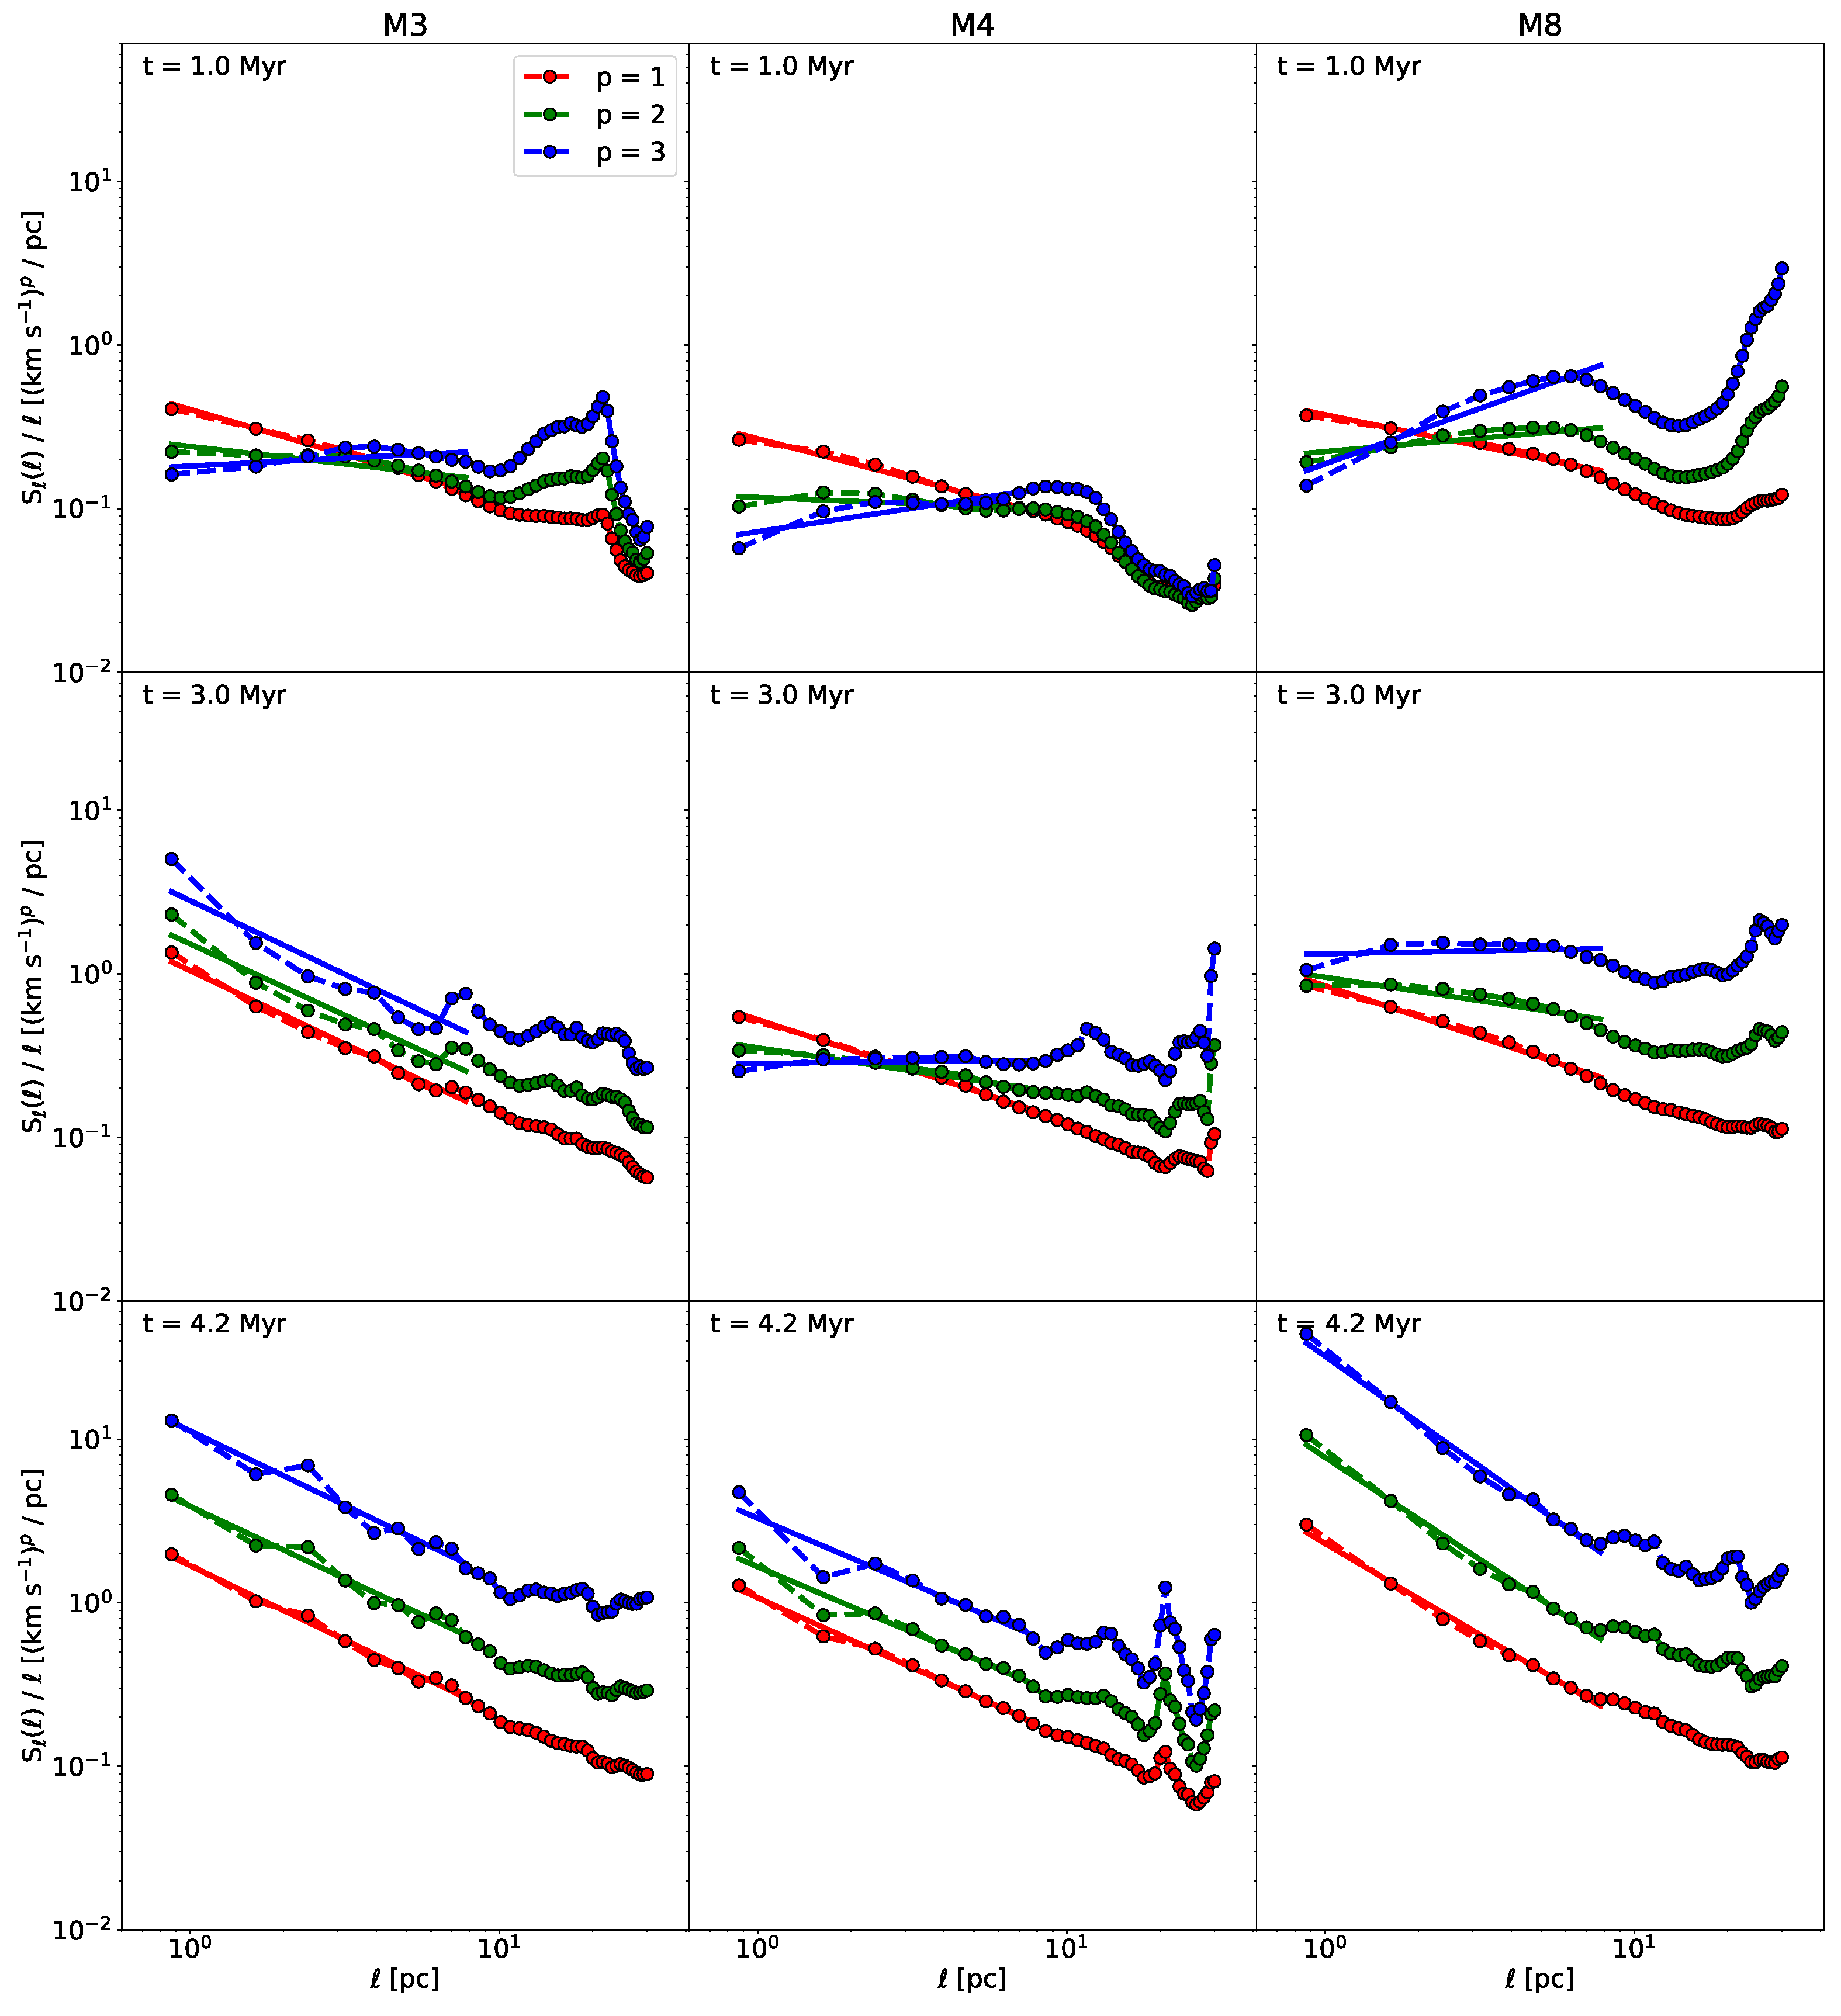
\includegraphics[width=\textwidth]{app_examples_wthres_sl_l.pdf}
    \caption{
        As Fig.~\ref{pic:results:vsf_example}, but plotting the relation between S$_{\ell}$ / $\ell$ as function of lag scale $l$ and order $p$.
    }
    \label{pic:appInertial:examples_with_threshold_sl_vs_l}
\end{figure*}
 	
 	
\begin{figure*}
    \centering
    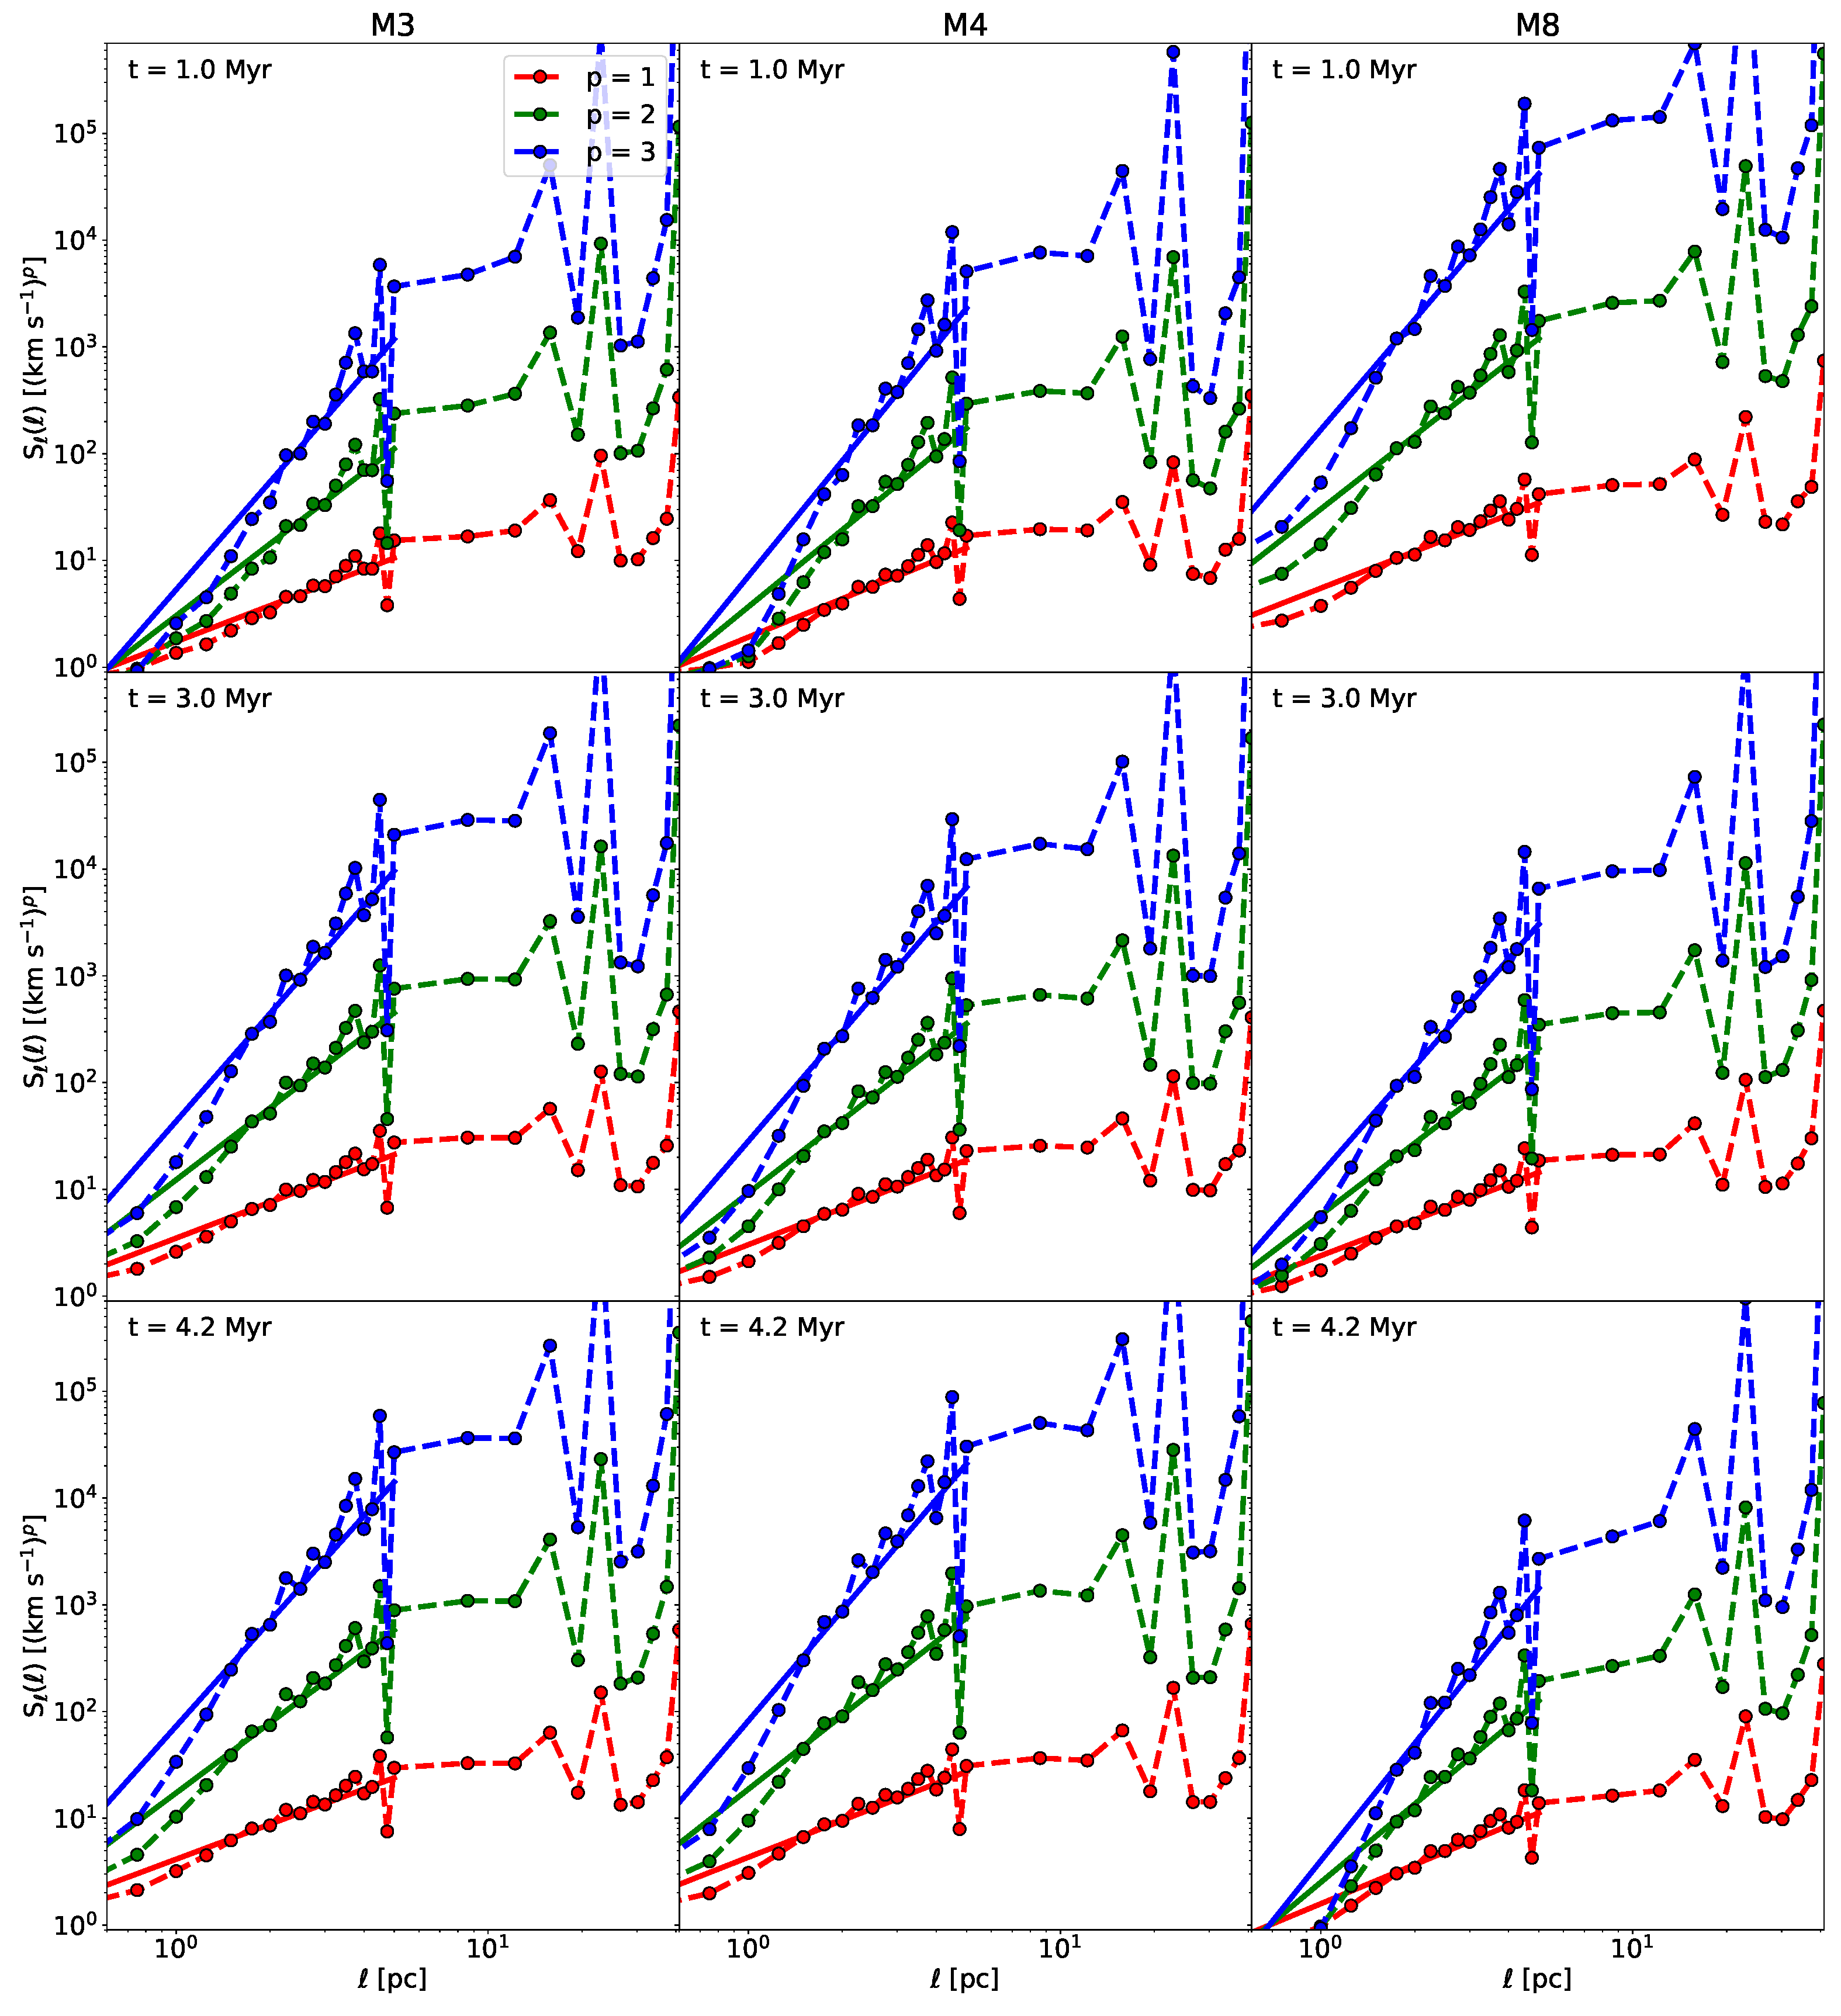
\includegraphics[width=\textwidth]{app_examples_woutthres_s_l.pdf}
    \caption{
        As Fig.~\ref{pic:results:vsf_example}, but based on data without density threshold.
    }
    \label{pic:appInertial:examples_without_threshold_s_vs_l}
\end{figure*}
 	
 	
\begin{figure*}
    \centering
    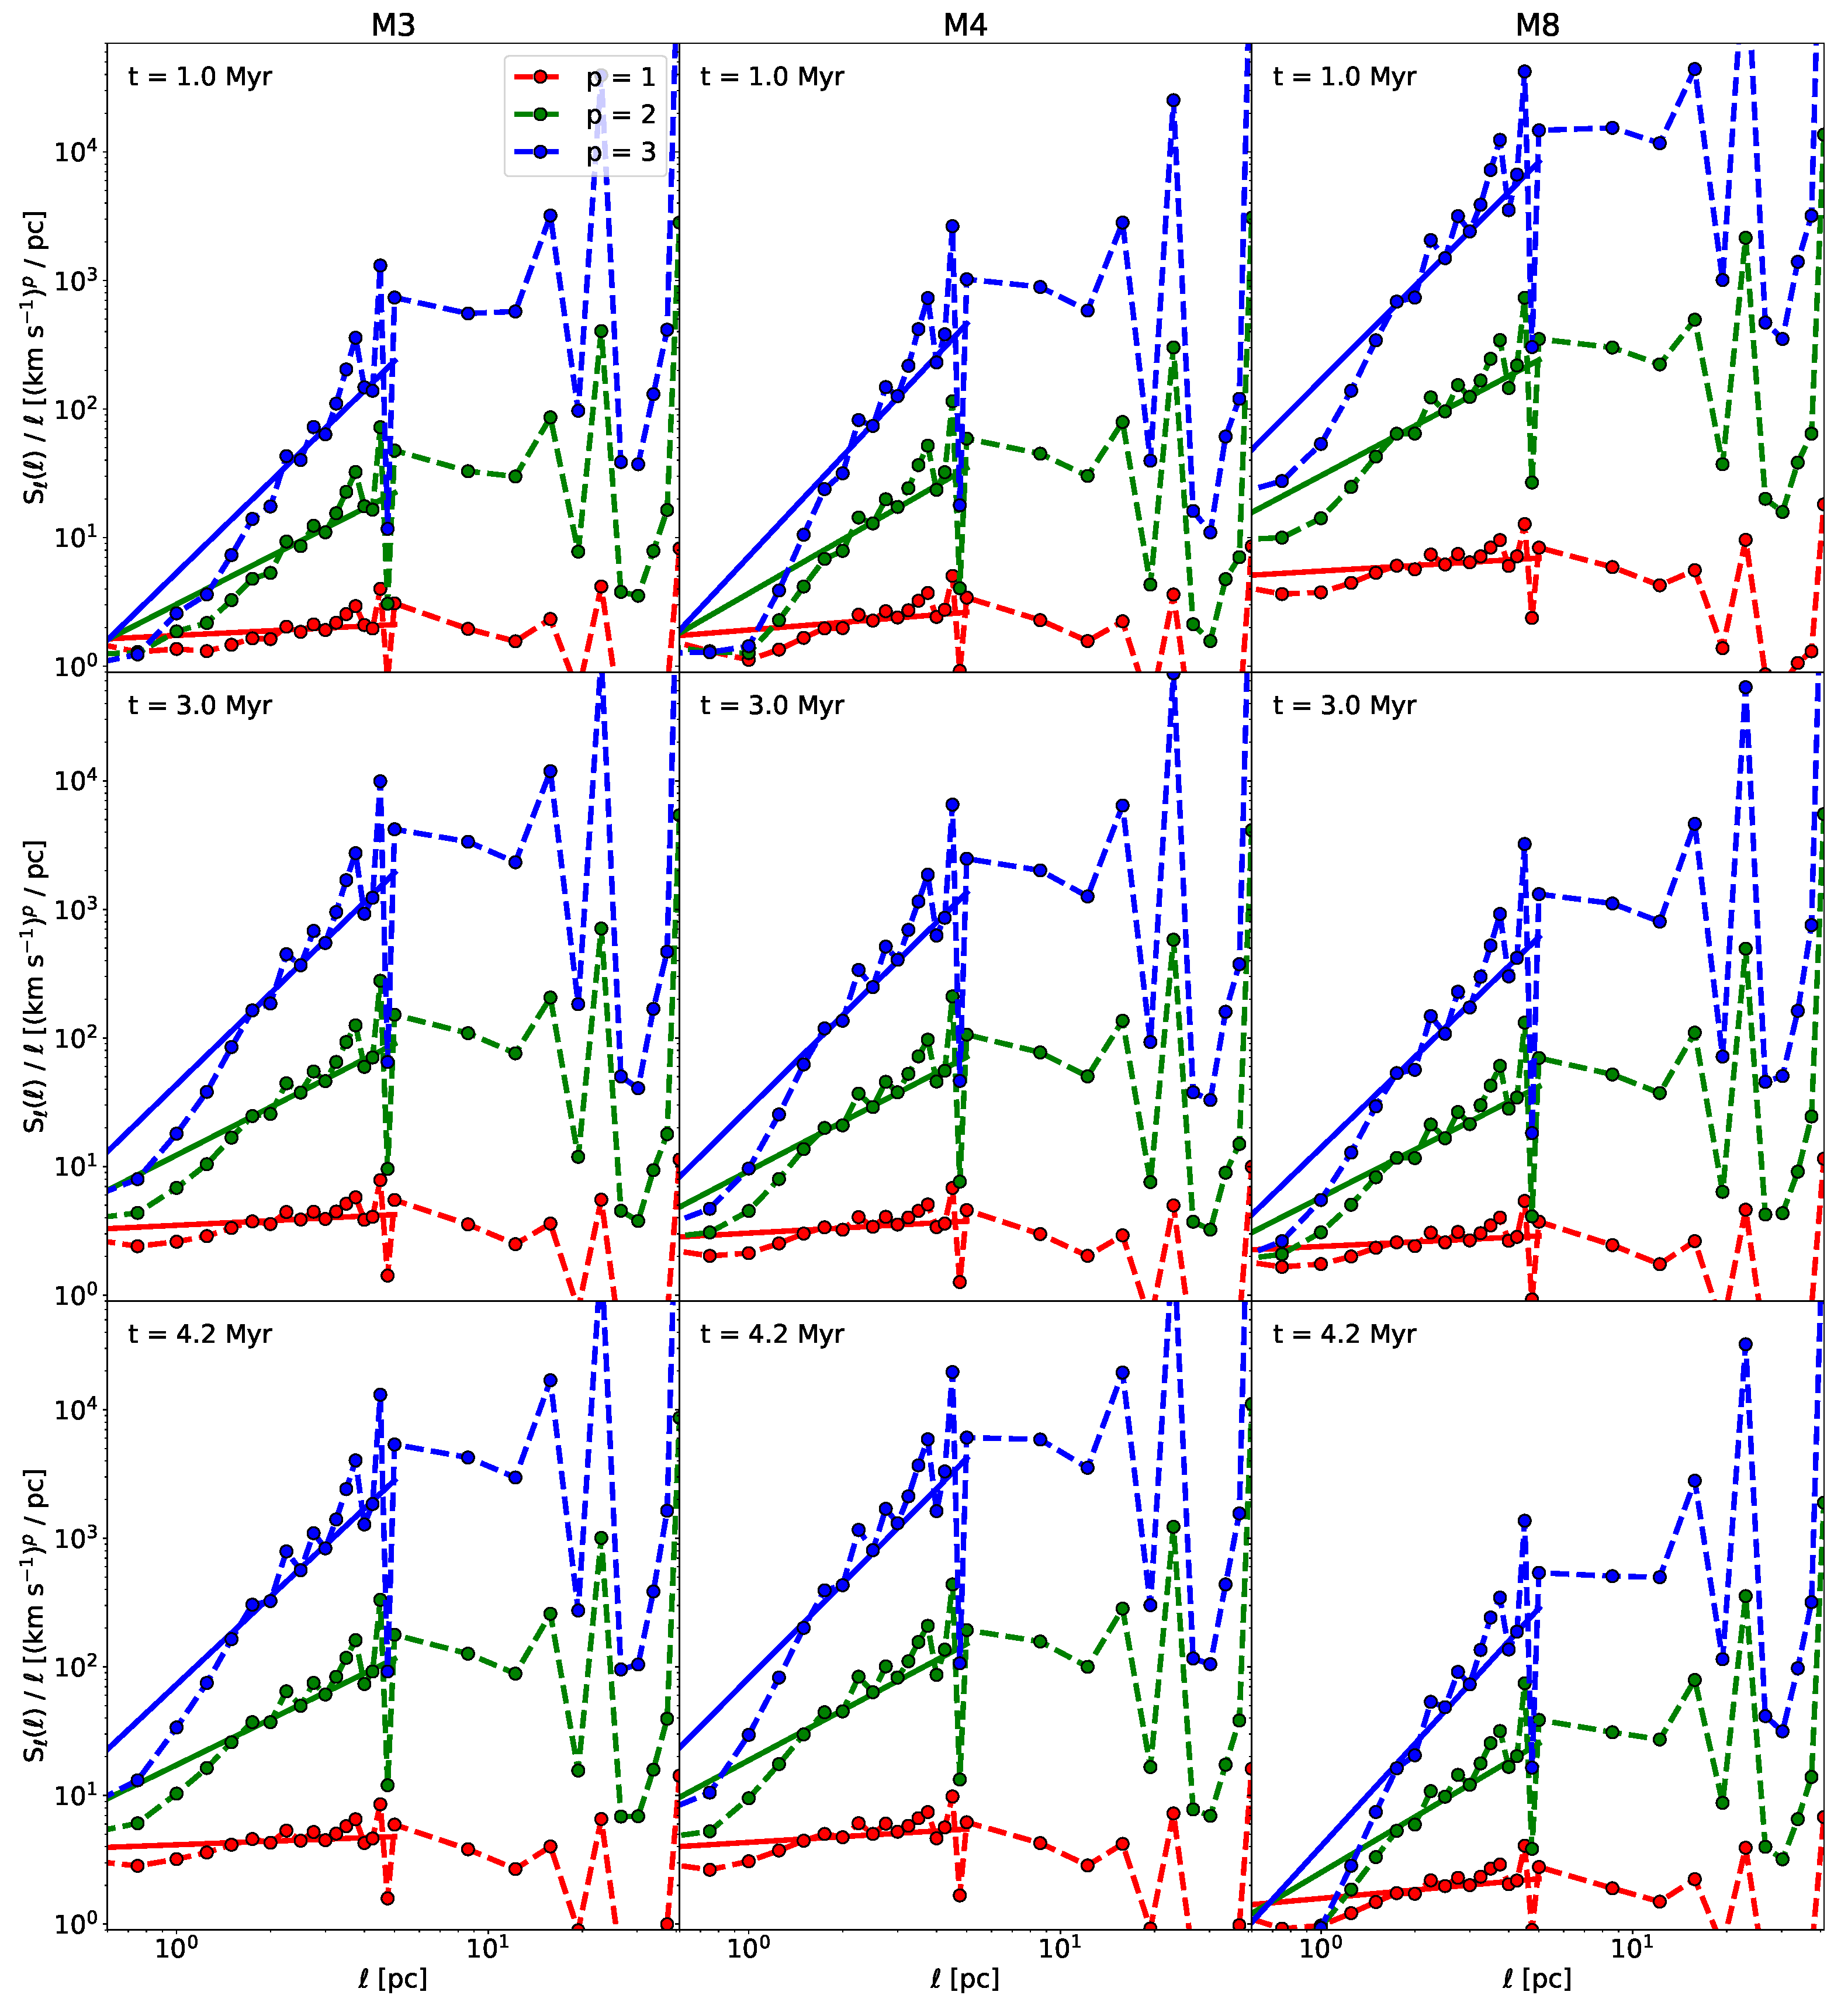
\includegraphics[width=\textwidth]{app_examples_woutthres_sl_l.pdf}
    \caption{
        As Fig.~\ref{pic:appInertial:examples_with_threshold_sl_vs_l}, but based on data without density threshold.
    }
    \label{pic:appInertial:examples_without_threshold_sl_vs_l}
\end{figure*}


 	
\begin{figure*}
    \centering
    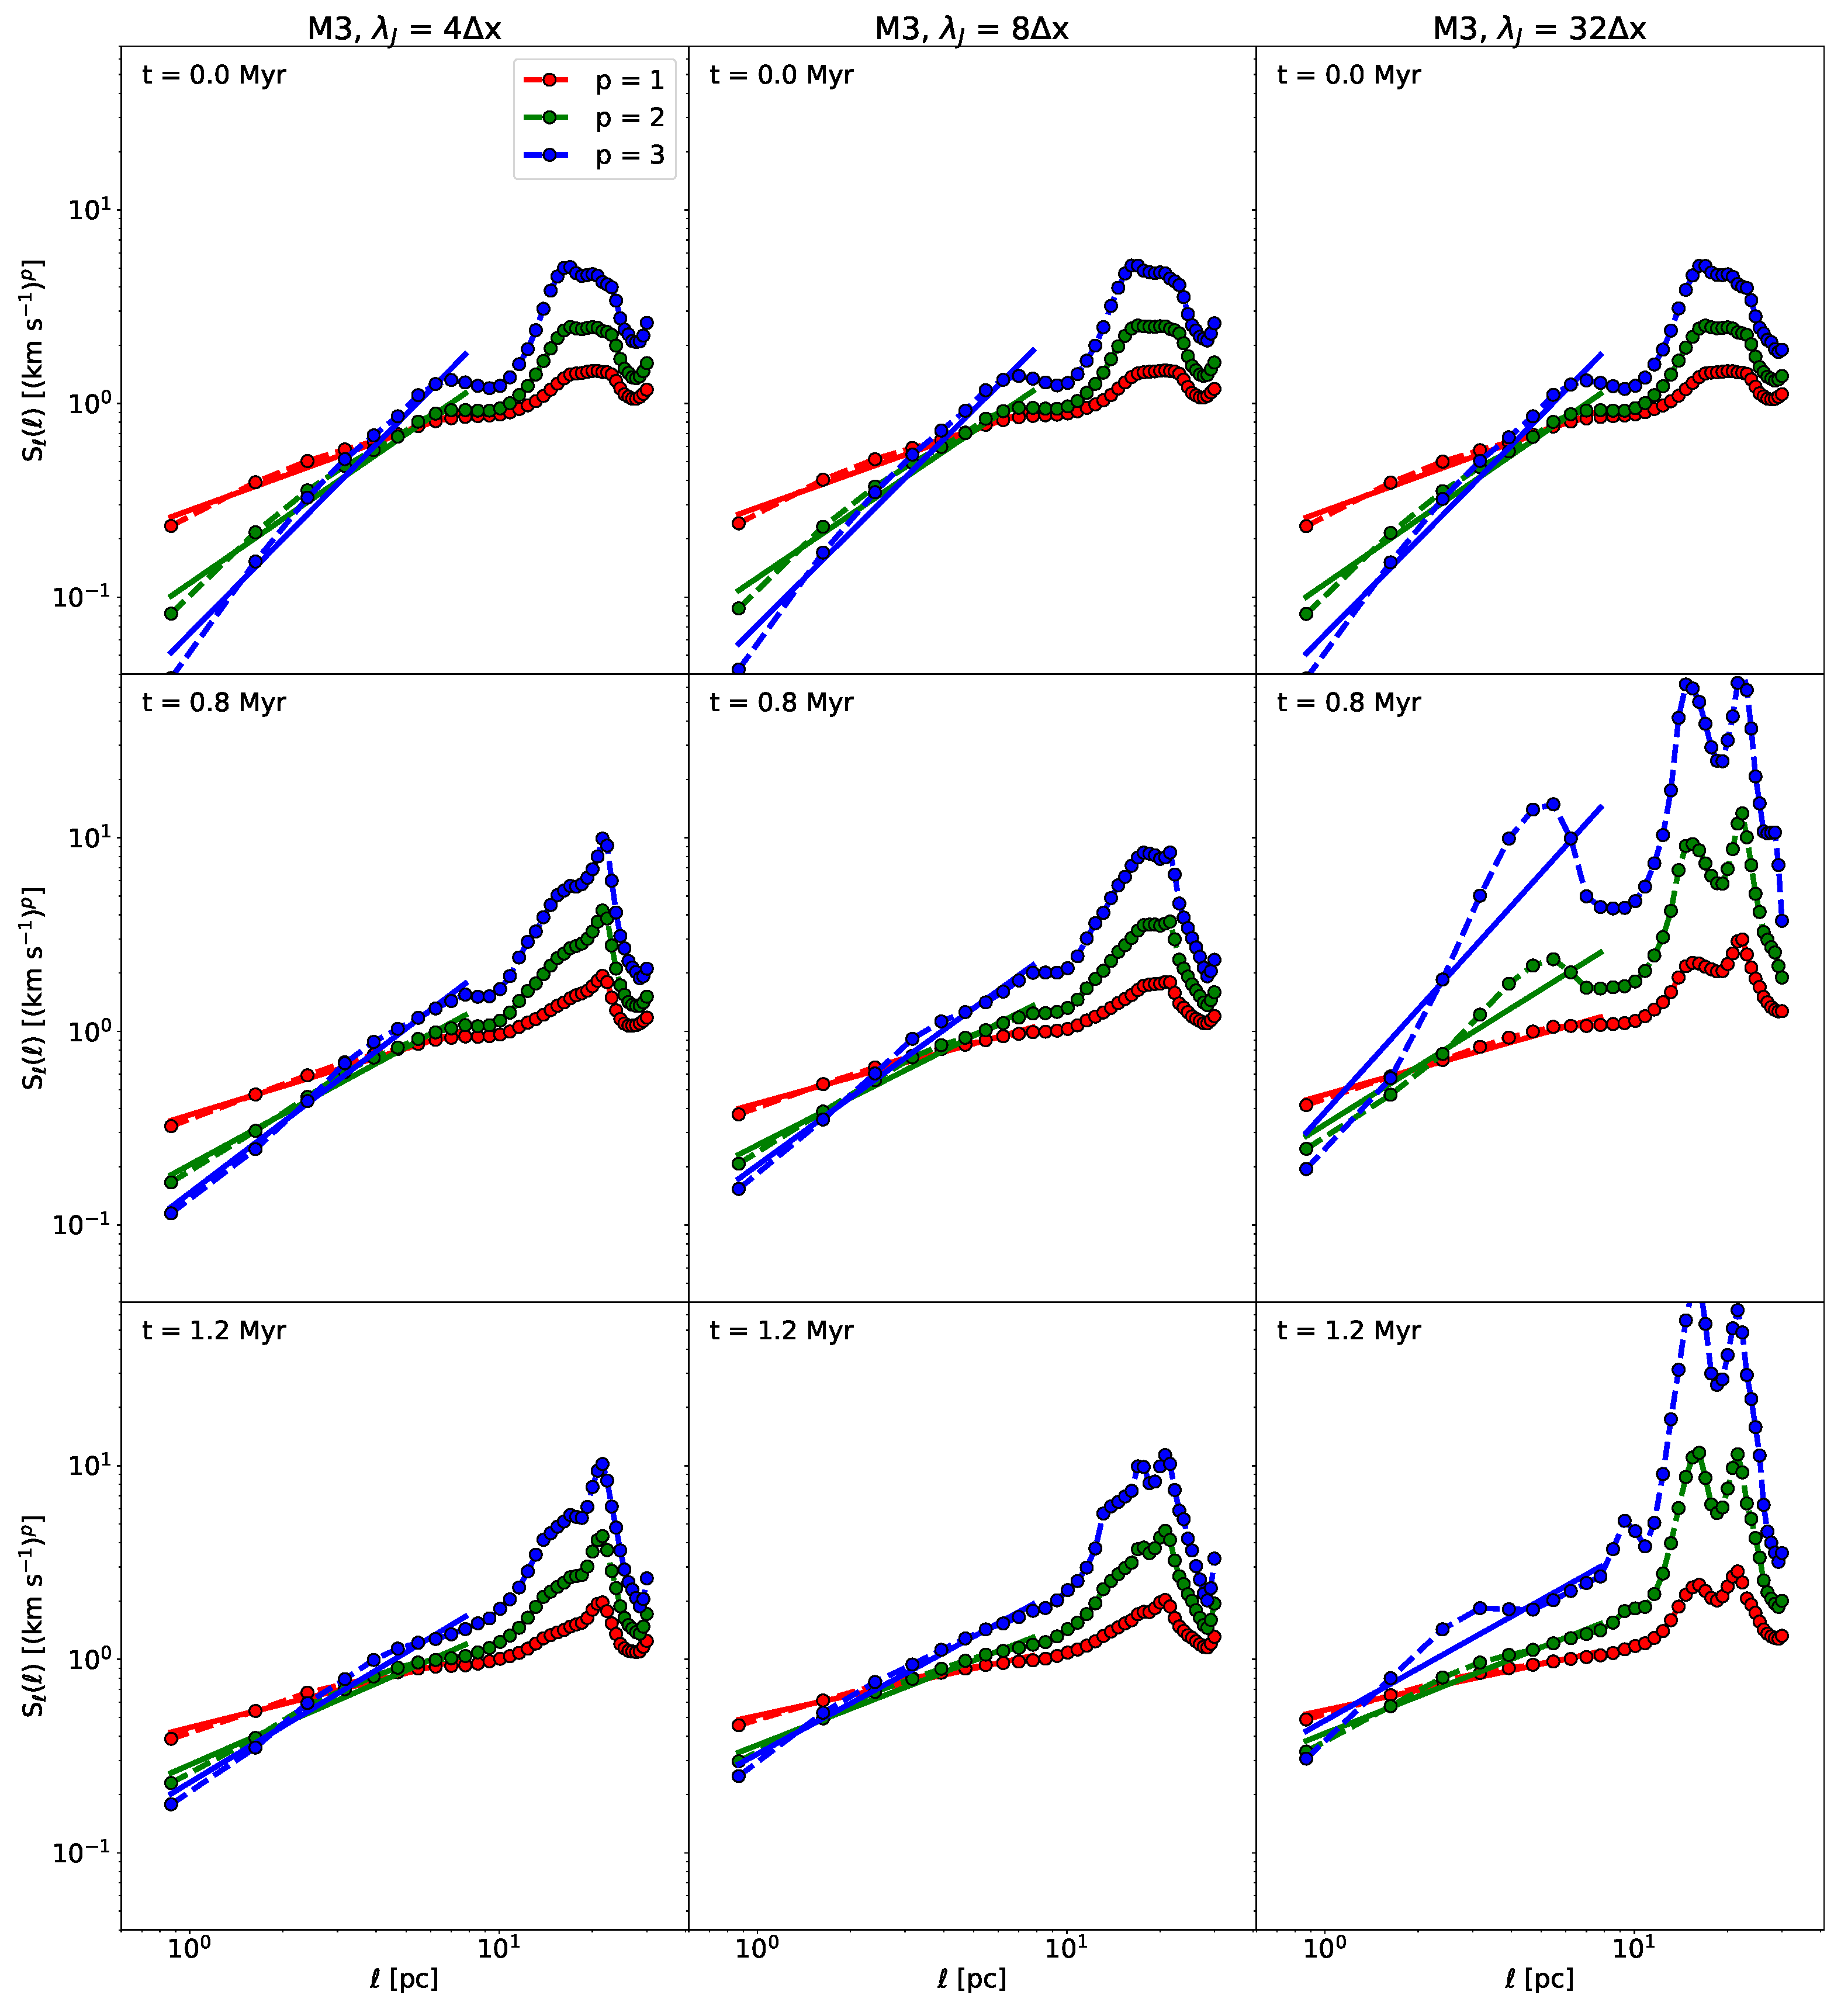
\includegraphics[width=\textwidth]{app_examples_jeans_s_l.pdf}
    \caption{
        The figures show additional examples of VSFs, based on data of \texttt{M3} with density threshold, at the different refinement levels (\textit{left} to \textit{right}) $\lambda$~=~4~$\Delta$x, $\lambda$~=~8~$\Delta$x, and $\lambda$~=~8~$\Delta$x as function of lag scale $\ell$ and order $p$. 
        The examples are given for three different time steps, namely (\textit{top} to \textit{bottom}) t~=~0.0~Myr, 0.8~Myr, and 1.2~Myr.
        The dots (connected by dashed lines) show the values computed from the simulations. 
        The solid lines represent the power-law relation fitted to the respective structure functions.
    }
    \label{pic:appInertial:examples_jeans_s_vs_l}
\end{figure*}


 	
\begin{figure*}
    \centering
    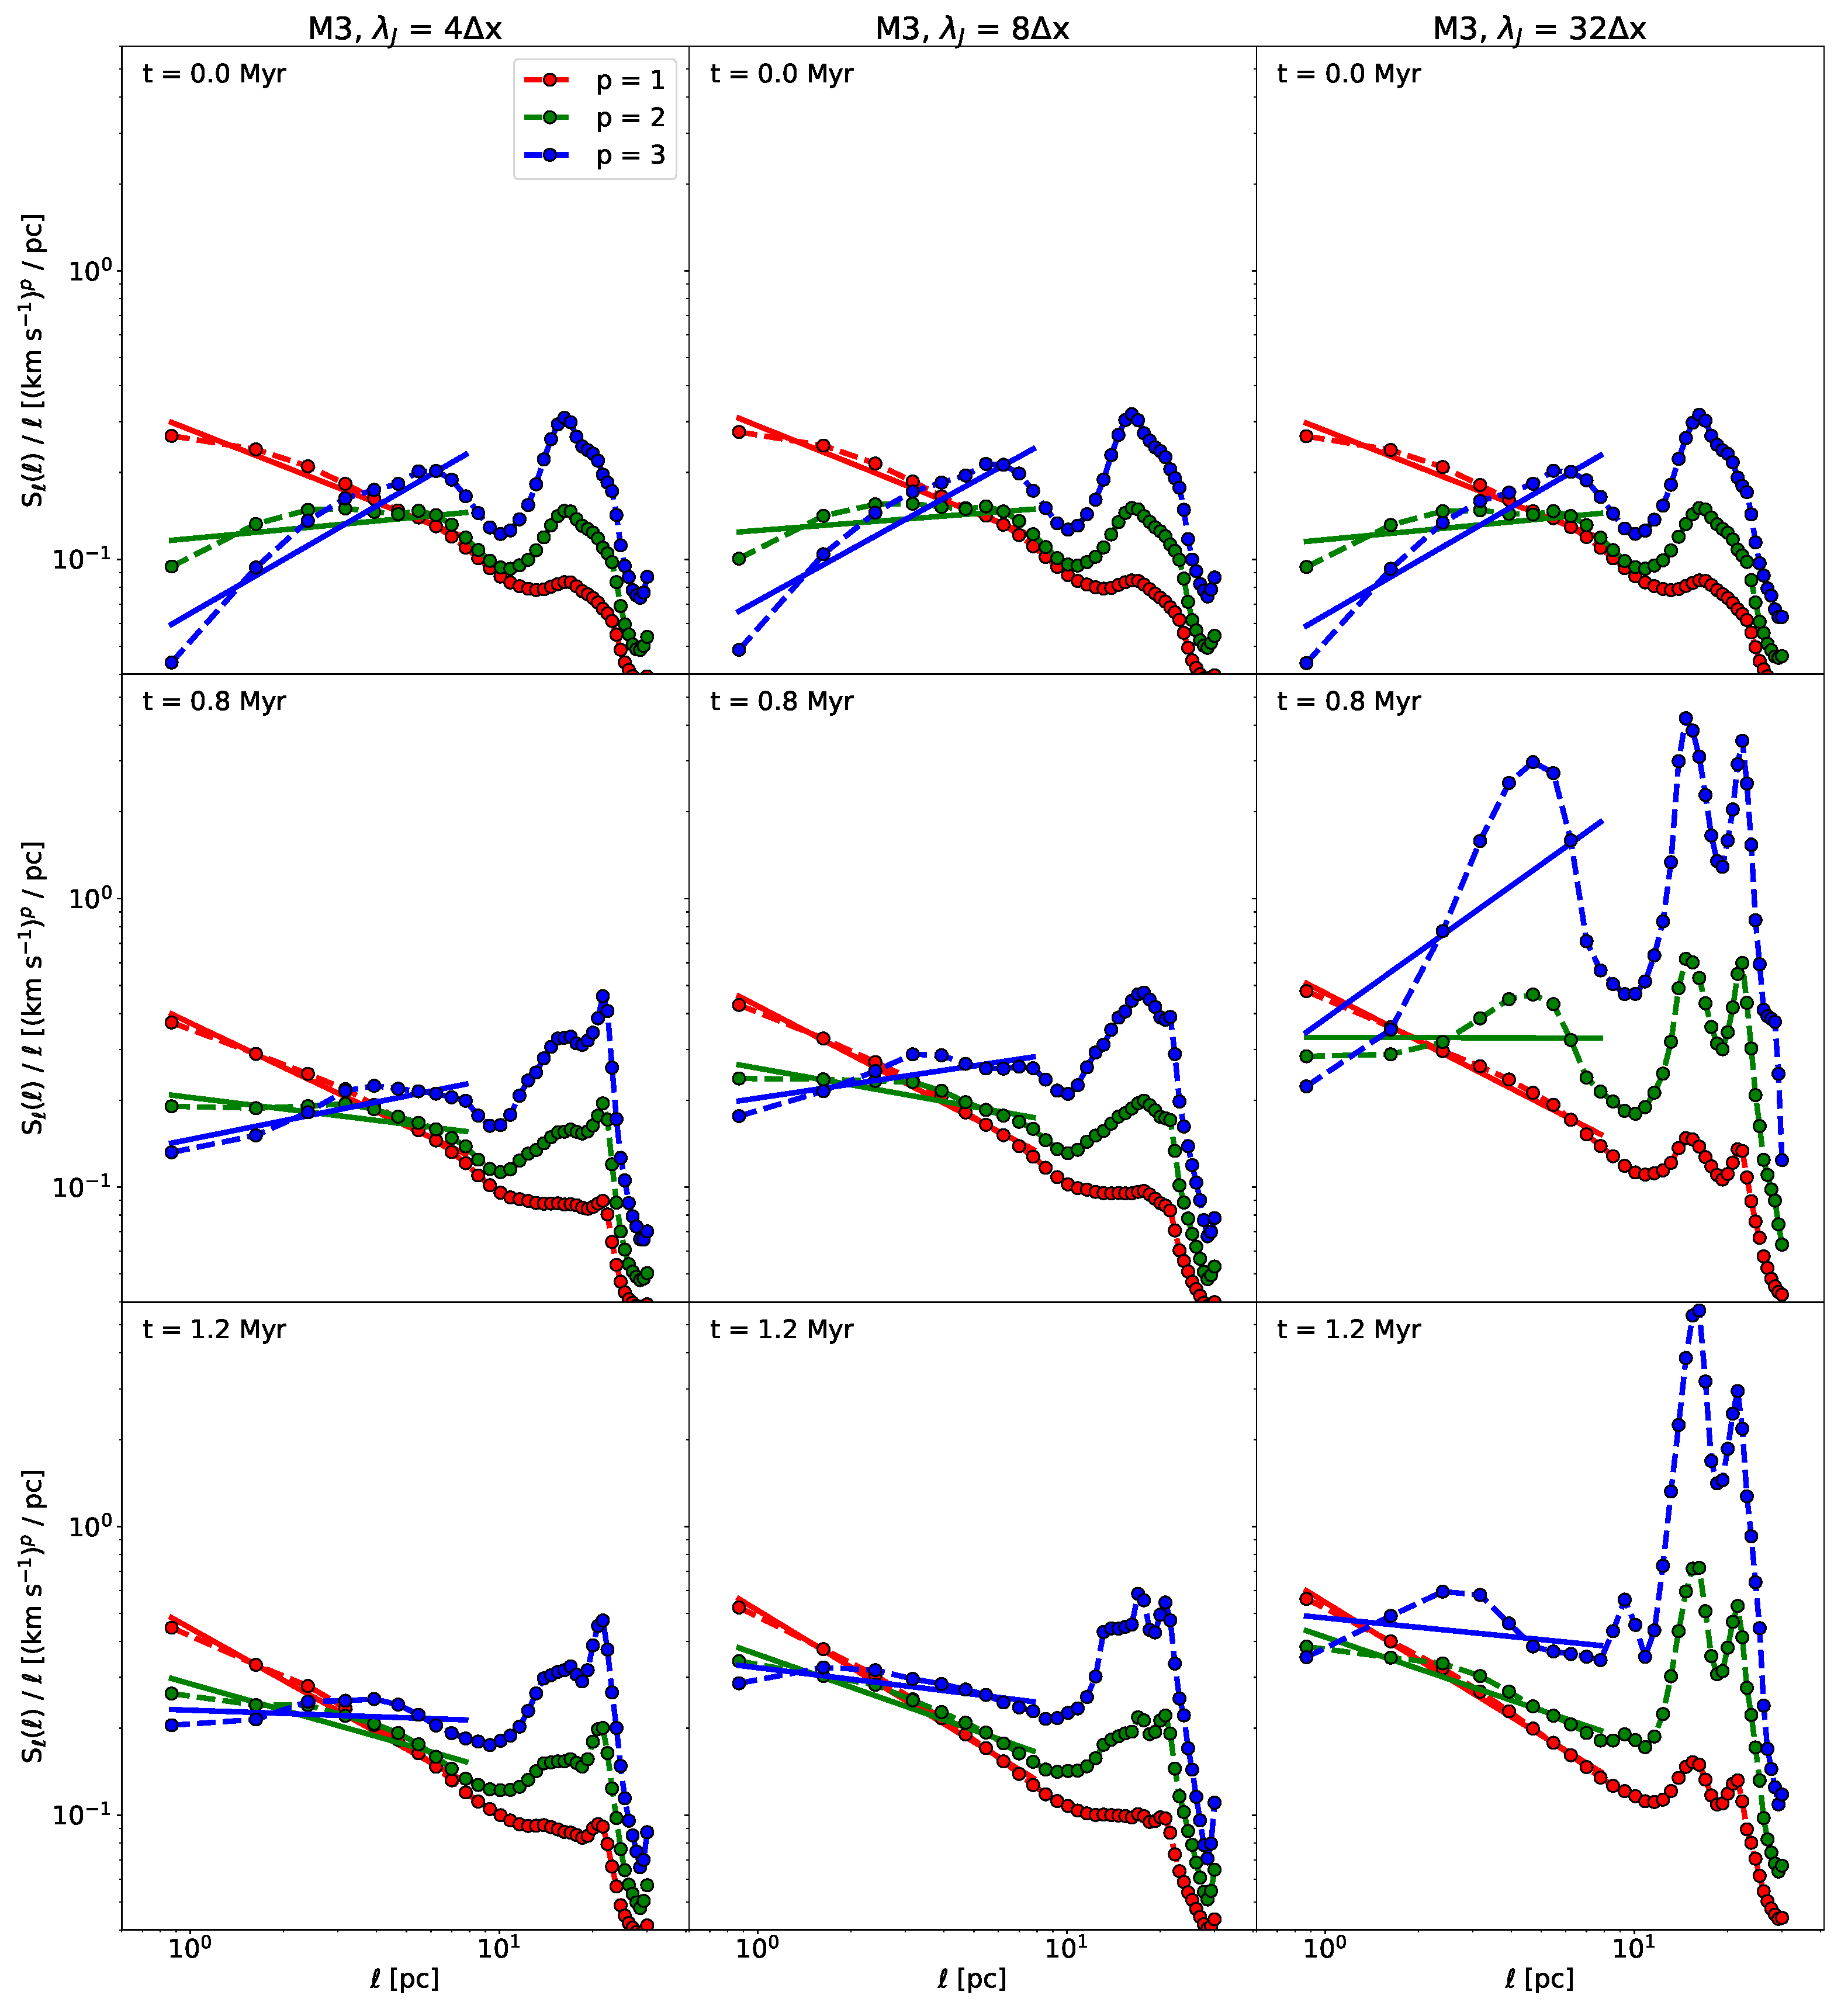
\includegraphics[width=\textwidth]{app_examples_jeans_sl_l.pdf}
    \caption{
        As Fig.~\ref{pic:appInertial:examples_jeans_s_vs_l}, but plotting the relation between S$_{\ell}$ / $\ell$ as function of lag scale $l$ and order $p$.
    }
    \label{pic:appInertial:examples_jeans_sl_vs_l}
\end{figure*}

\subsection{Standard Analysis}\label{Bsub:standard}

\textbf{
\ref{pic:appInertial:examples_with_threshold_sl_vs_l} extends the data presented in Sect.~\ref{results:normal} and discussed in Sect.~\ref{discussion:normal}.
The figure uses the same format as Fig.~\ref{pic:results:vsf_example}.
}
The straight lines within the plots indicate the power-law relation that we have fitted onto the VSFs, considering the range 0.8~$\leq\,\ell\,\leq$~8~pc.

We see that in most of the cases the VSFs are in good agreement with the described power-law relation within the fitted ranges (e.g., Fig.~\ref{pic:results:vsf_example}). 
However, there are cases when the VSF is not well reproduced by a simple, single power-law function, such as \texttt{M3} at $t=3.0$~Myr in Fig.~\ref{pic:results:vsf_example}.
This appears to occur particularly when the dominant mechanism driving turbulence changes from large-scale driving to internal contraction. 
At this point the  larger scales of the clouds (larger~$\ell$) are still dominated by external driving, while the smaller scales (smaller~$\ell$) start to accelerate mostly due to gravitational fragmentation and infall motions.
The consequence is that the actual VSF is a superposition of two processes that amplify the relative motions of the gas differently and on different scales.
A single power-law cannot describe this scenario adequately. 


\subsection{No Density Threshold} \label{Bsub:full}

Figs.~\ref{pic:appInertial:examples_without_threshold_s_vs_l} and~\ref{pic:appInertial:examples_without_threshold_sl_vs_l} extend the set of VSFs for the box without a density threshold presented in Sect.~\ref{results:densthres} and discussed in Sect.~\ref{discussion:densthres}.

Here we also find problems describing the behaviour of small-scale motions with $\ell\,\lesssim$~2~pc.
In this case we primarily capture the turbulent motions within the low-density ISM. 
Contrary to the modelled MCs, the ISM is not organised in hierarchical structures, and the turbulence within the ISM is predominantly driven by SN explosions.
These produce structured correlations at the large scales of entire blast waves as well as the small scales across shock fronts.
Yet, we see that we can fit the VSFs with a power law within the intermediate lag scale ranges (2~pc~$\lesssim\,\ell\,\lesssim$~8~pc), suggesting this range of length scales is dominated by a turbulent cascade.



\subsection{Varying Refinement} \label{Bsub:Jeans}

Figs.~\ref{pic:appInertial:examples_jeans_s_vs_l} and~\ref{pic:appInertial:examples_jeans_sl_vs_l} extend the set of VSFs presented for clouds with varying amounts of refinement in gravitationally collapsing regions in Sect.~\ref{results:refinement} and discussed in Sect.~\ref{discussion:refinement}.

A final example of VSFs not following a power law at intermediate scales is given by cloud \texttt{M3} at $t=0.8$~Myr and with $\lambda_\mathrm{J} = 32\Delta x$ in Fig.~\ref{pic:appInertial:examples_jeans_s_vs_l}.
This represents the VSF of a cloud that is interacting with a SN blast wave.
In this case the maximal amplification is neither at the scale of the cloud, where the turbulence is driven by external sources, nor on small scales where gravitational contraction acts.
Instead the local maximum is the intermediate scale. 
Considering the morphology of the cloud and the cloud's environment this can only occur when the shock front of a SN is currently propagating through the cloud. 
Thus, the VSF here is a superposition of three driving mechanisms:
first, the external large-scale driving; second, self-gravity that leads to contractive motions; and finally the shock jump that injects kinetic energy as it moves through the cloud. 
The effect of the shock, however, is only local and short-lived as the injected turbulence decays quickly (compare with \texttt{M3} at $t=1.2$~Myr and with $\lambda_\mathrm{J} = 32\Delta x$ in Fig.~\ref{pic:appInertial:examples_jeans_s_vs_l}).












